%%%%%%%%%%%%%%%%%%%%%%%%%%%%%%%%%%%%%%%%%%%%%%%%%%%%%%%%
%%%%%%%%%%%%%%%%%%%%%%%%%%%%%%%%%%%%%%%%%%%%%%%%%%%%%%%%
\section{Fast Interpretable Greedy-Tree Sums (\figs)}
\label{class:FIGS}

Fast Interpretable Greedy-Tree Sums (\figs) \cite{FIGS,G-FIGS}
is an extension of the basic CART structure introduced in \cref{class:CART}.
Depending on the nature of the training data,
a CART will tend to reproduce subsets of the tree along different branches.
The resulting deep trees are not ideal as they contain many splits,
increasing the chance of fitting to noise in the data,
and because they have less data to work with at each subsequent split,
increasing the variance of the tree's predictions.

\figs improves upon the iterative training process of CART
by considering adding the next split as the root of a new tree $f_{t}$,
in addition to adding the next split at the bottom of an existing tree.
This reduces the number of splits when the data has an additive structure,
as can be seen in \cref{fig:FIGS:intro}, thereby also increasing the interpretability.
The splits are chosen greedily according to the usual splitting criteria;
typically the Gini impurity of \cref{class:CART:gini_impurity} is used for classification\footnote{The
Gini feature importance of \cref{ml_general:interp:feature_importance:MDI}
can also be computed across \figs trees, see
\texttt{imodels} PR \href{https://github.com/csinva/imodels/pull/154}{\#154}.}.

During training, each tree $k$ is fit to the residuals remaining after summing the other tree's predictions,
$r_{i}^{\left(-k\right)}$ \cref{eq:FIGS:FIGS_eqs:r}.
The predicted weight $w_{l,\,k}$ \cref{eq:FIGS:FIGS_eqs:weight} at each leaf $l$ of tree $k$
are found by taking the mean of the $r_{i}^{\left(-k\right)}$ residuals, from the other trees,
over the $\vb{x}_{i}$ data points $\left\{l\right\}$ that reach the leaf.
Note that when there are no other trees,
\eg when growing the first tree or if the data is non-additive,
the sum $\sum_{t \neq k} f_{t}$ will be zero and $r_{i}^{\left(-k\right)} = y_{i}$.
In this case, the leaf weights are simply $w_{l} = n_{l,\,1}/n_{l}$,
\ie the proportion of positive $y_{i} = 1$ data points in leaf $l$.
Finally, the predictions for the trained model are made by
summing the relevant leaf weight $w_{l,k}\left(\vb{x}_{i}\right)$ from each tree,
and then taking the sigmoid\footnote{See
\texttt{imodels} PR \href{https://github.com/csinva/imodels/pull/150}{\#150}
and \cref{ml_general:calibration:platt:sigmoid}
for more.} of the result
to constrain the output between \num{0} and \num{1}.
See \cref{algo:FIGS:fit_algo} for an outline of the training algorithm.

\begin{subequations}\label{eq:FIGS_eqs}
\begin{align}
r_{i}^{\left(-k\right)} &= y_{i} - \sum_{t \neq k} f_{t}\left(\vb{x}_{i}\right) \label{eq:FIGS:FIGS_eqs:r} \\
w_{l,\,k} &= \frac{1}{\abs{\left\{l\right\}}} \sum_{i \in \left\{l\right\}} r_{i}^{\left(-k\right)} \label{eq:FIGS:FIGS_eqs:weight}
\end{align}
\end{subequations}

\begin{figure}[H]
\centering
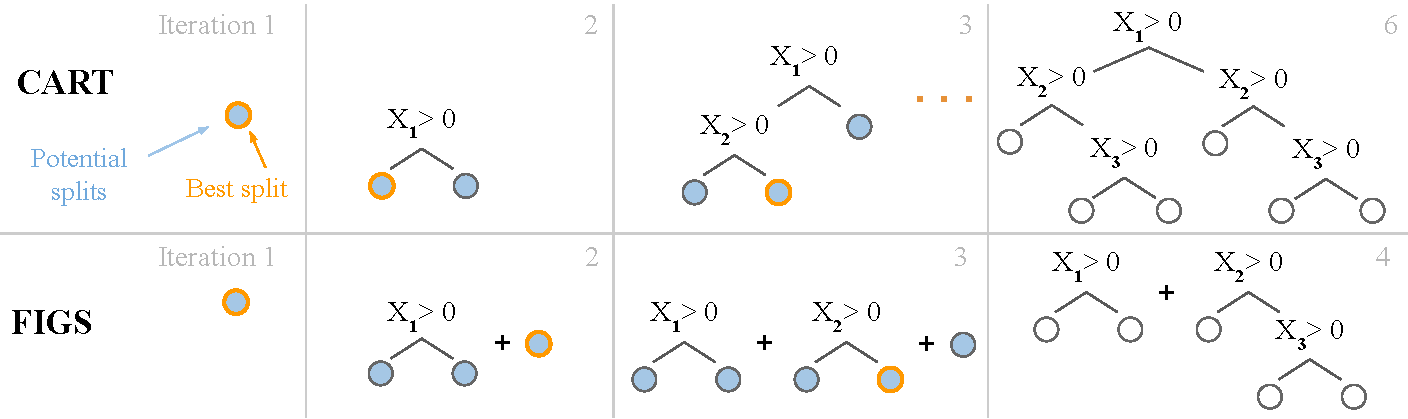
\includegraphics[width=\textwidth]{figures/ml/figs_intro_fig}
\caption{
A comparison of CART and \figs tree growth on the toy dataset
$y = \identity_{x_{1} > 0} + \identity_{x_{2} > 0} \, \identity_{x_{3} > 0}$ \cite{FIGS}.
At each training iteration \figs considers adding a new split at the bottom of the existing tree(s) like CART,
but also considers starting a new tree entirely.
Notice that CART must repeat the $x_{2}, x_{3}$ subtree on each side of the $x_{1}$ split,
while \figs captures the additive structure of $y$ directly, thereby saving \num{2} splits.
}
\label{fig:FIGS:intro}
\end{figure}

\begin{algorithm}[h]
  \caption{\figs fitting algorithm, adapted from \cite{FIGS}.}
  \label{algo:FIGS:fit_algo}
  \small
\begin{algorithmic}
  \State {\figs}(X: features, y: outcomes, $\nu$: max\_splits, $k_{\text{max}}$: max\_trees)
  \State trees = []
  \While{count\_total\_splits(trees) $< \nu$ and count(trees) $< k_{\text{max}}$:}
    \State all\_trees = join(trees, build\_new\_tree()) \textcolor{codegreen}{\# add new tree}
    \State potential\_splits = []
    \For{}\hspace{-3pt}tree in all\_trees:
        \State y\_residuals = y $-$ predict(all\_trees except tree)
        \For{}\hspace{-3pt}leaf in tree:
            \State potential\_split = split(X, y\_residuals, leaf)
            \State potential\_splits.append(potential\_split)
        \EndFor
    \EndFor
    \State best\_split = split\_with\_min\_impurity(potential\_splits)
    \State trees.insert(best\_split)
  \EndWhile
\end{algorithmic}
\end{algorithm}

The resulting \figs model is thus an ensemble of CART-like trees,
similar to the BDT and RF models of \cref{class:BDT,class:RF}.
However, \figs can explicitly capture any additive structure present in the data,
while the ensemble trees of the BDT (RF) model being trained sequentially (independently) can not.
Rather than constraining the depth or number of trees separately like other tree-based models,
\figs can impose a limit on the total number of splits across all trees via the hyperparameter $\nu$.
This makes the construction of small, interpretable, models much easier.
Similar to CART, \figs can also set hyperparameters for
the minimum decrease in impurity and
number of features to consider at each split.
Additionally, the number of trees can  be independently constrained\footnote{See
\texttt{imodels} PR \href{https://github.com/csinva/imodels/pull/153}{\#153}.} via
the hyperparameter $k_{\text{max}}$.

With $\nu < 20$, readily interpretable \figs models have been observed
to have state-of-the-art performance on multiple datasets \cite{FIGS}.
A \python implementation of the \figs algorithm can be found in the \texttt{imodels} package \cite{imodels}.
The \figs training time goes as $\order{n \, \nu^{2} m^{2}}$ \cite{FIGS},
where $n$ is the number of features and $m$ is the number of data points,
which is quite fast on a modern machine for reasonable $m$, even when $n$ is large.

A demonstration of \figs versus \xgboost, \cref{class:BDT:xgboost},
on a synthetic dataset containing additive structure
is provided in the \texttt{figs\_demo.ipynb} \href{https://github.com/mepland/data_science_notes/blob/main/plots/figs_demo.ipynb}{notebook}.
Visualizations of the three trees of the trained \figs model can be found in \cref{fig:FIGS:demo_trees}.
The \figs model has $\SI{8.4}{\percent}$ lower performance, as measured by ROC AUC, when compared to the \xgboost model.
However, the \figs model is much more interpretable,
using only \num{30} splits (\num{3} trees) versus \num{1496} splits (\num{64} trees) used by \xgboost,
a reduction of \SI{4887}{\percent} (\SI{2033}{\percent})!

The demonstration training dataset was created from two Monte Carlo (MC) generators, $i=0,1$,
combined with a logical \texttt{AND} on $\vb{y}_{i}$.
The features were labeled $\texttt{x\_i\_j}$ to indicate the originating MC generator.
In this case\footnote{The degree of separation between MC generators
\figs can achieve depends on the random seed and MC parameters.
Values that showed good separation were chosen here to illustrate
the power of \figs on additive data,
but further study is needed to quantify this behavior.},
the \figs model was able to discern the additive structure,
as can be seen by the general separation of the \texttt{x\_i\_j} features by $i$ between the \num{3} trees.
Lastly, with its constrained splits \figs is naturally more regularized than \xgboost,
as can be seen in the ROC curves of \cref{fig:FIGS:demo_roc:figs},
which should lead to less generalization error in production usage.

\newpage

\begin{landscape}
\begin{figure}[H]
  \centering
  \begin{subfigure}[b]{0.32\linewidth}\centering
      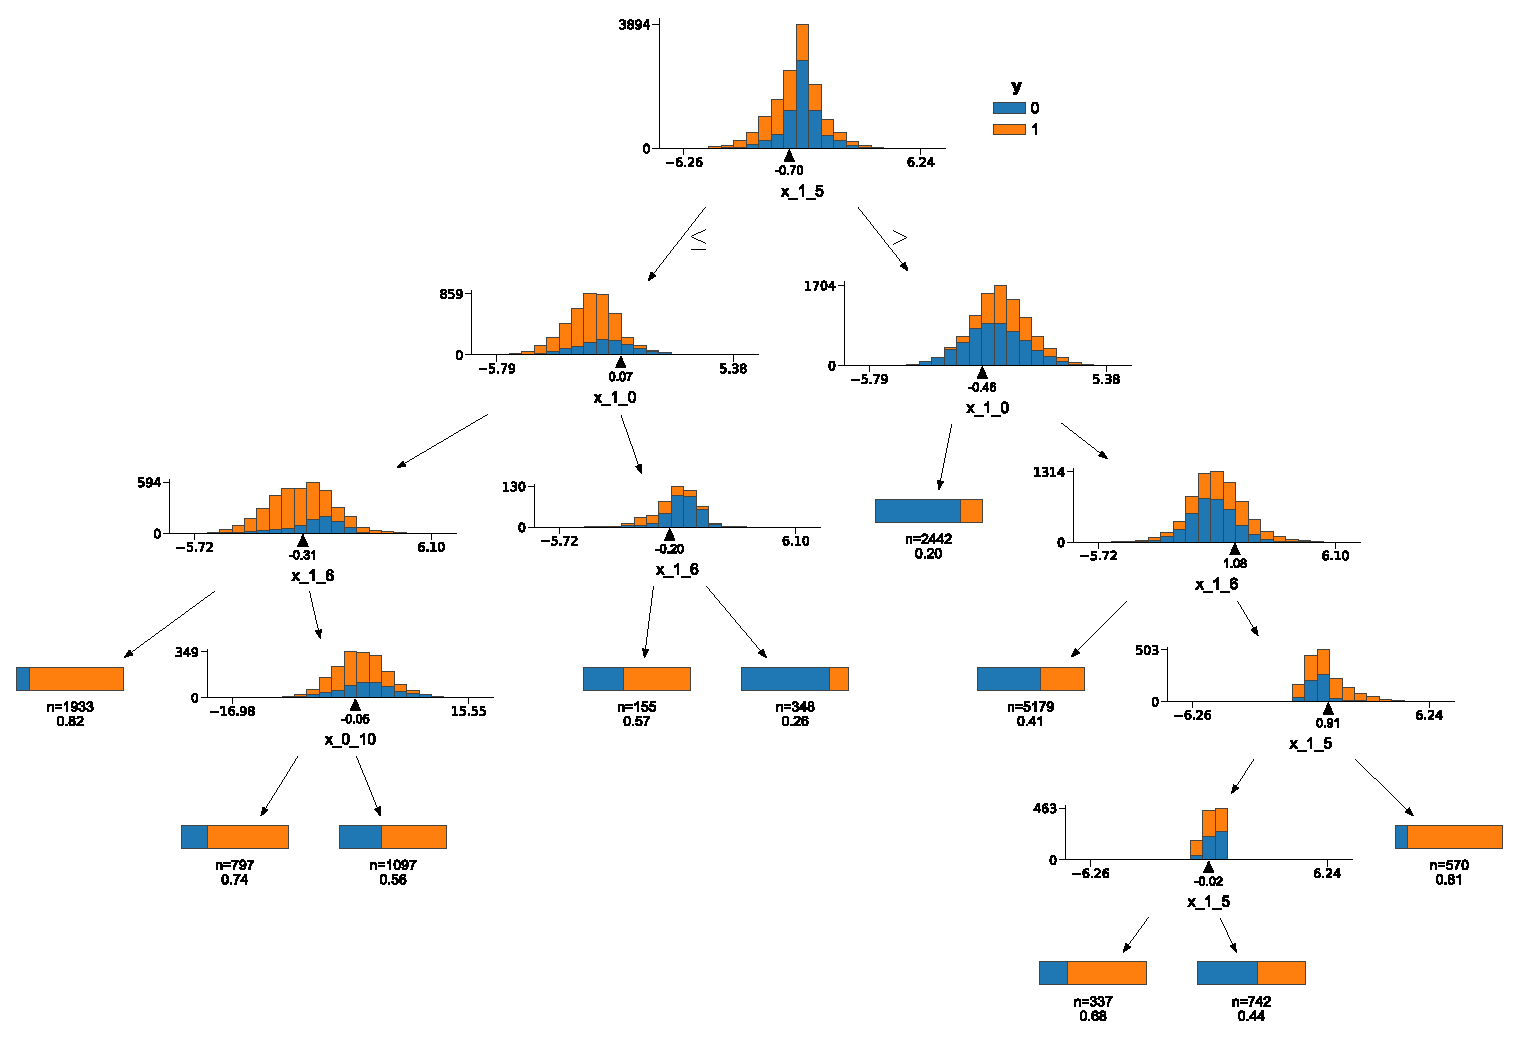
\includegraphics[width=\textwidth]{figures/ml/figs_demo/dtreeviz_figs_0}
  \caption{Tree 0}
  \label{fig:FIGS:demo_trees:tree0}
  \end{subfigure}
  ~
  \begin{subfigure}[b]{0.32\linewidth}\centering
      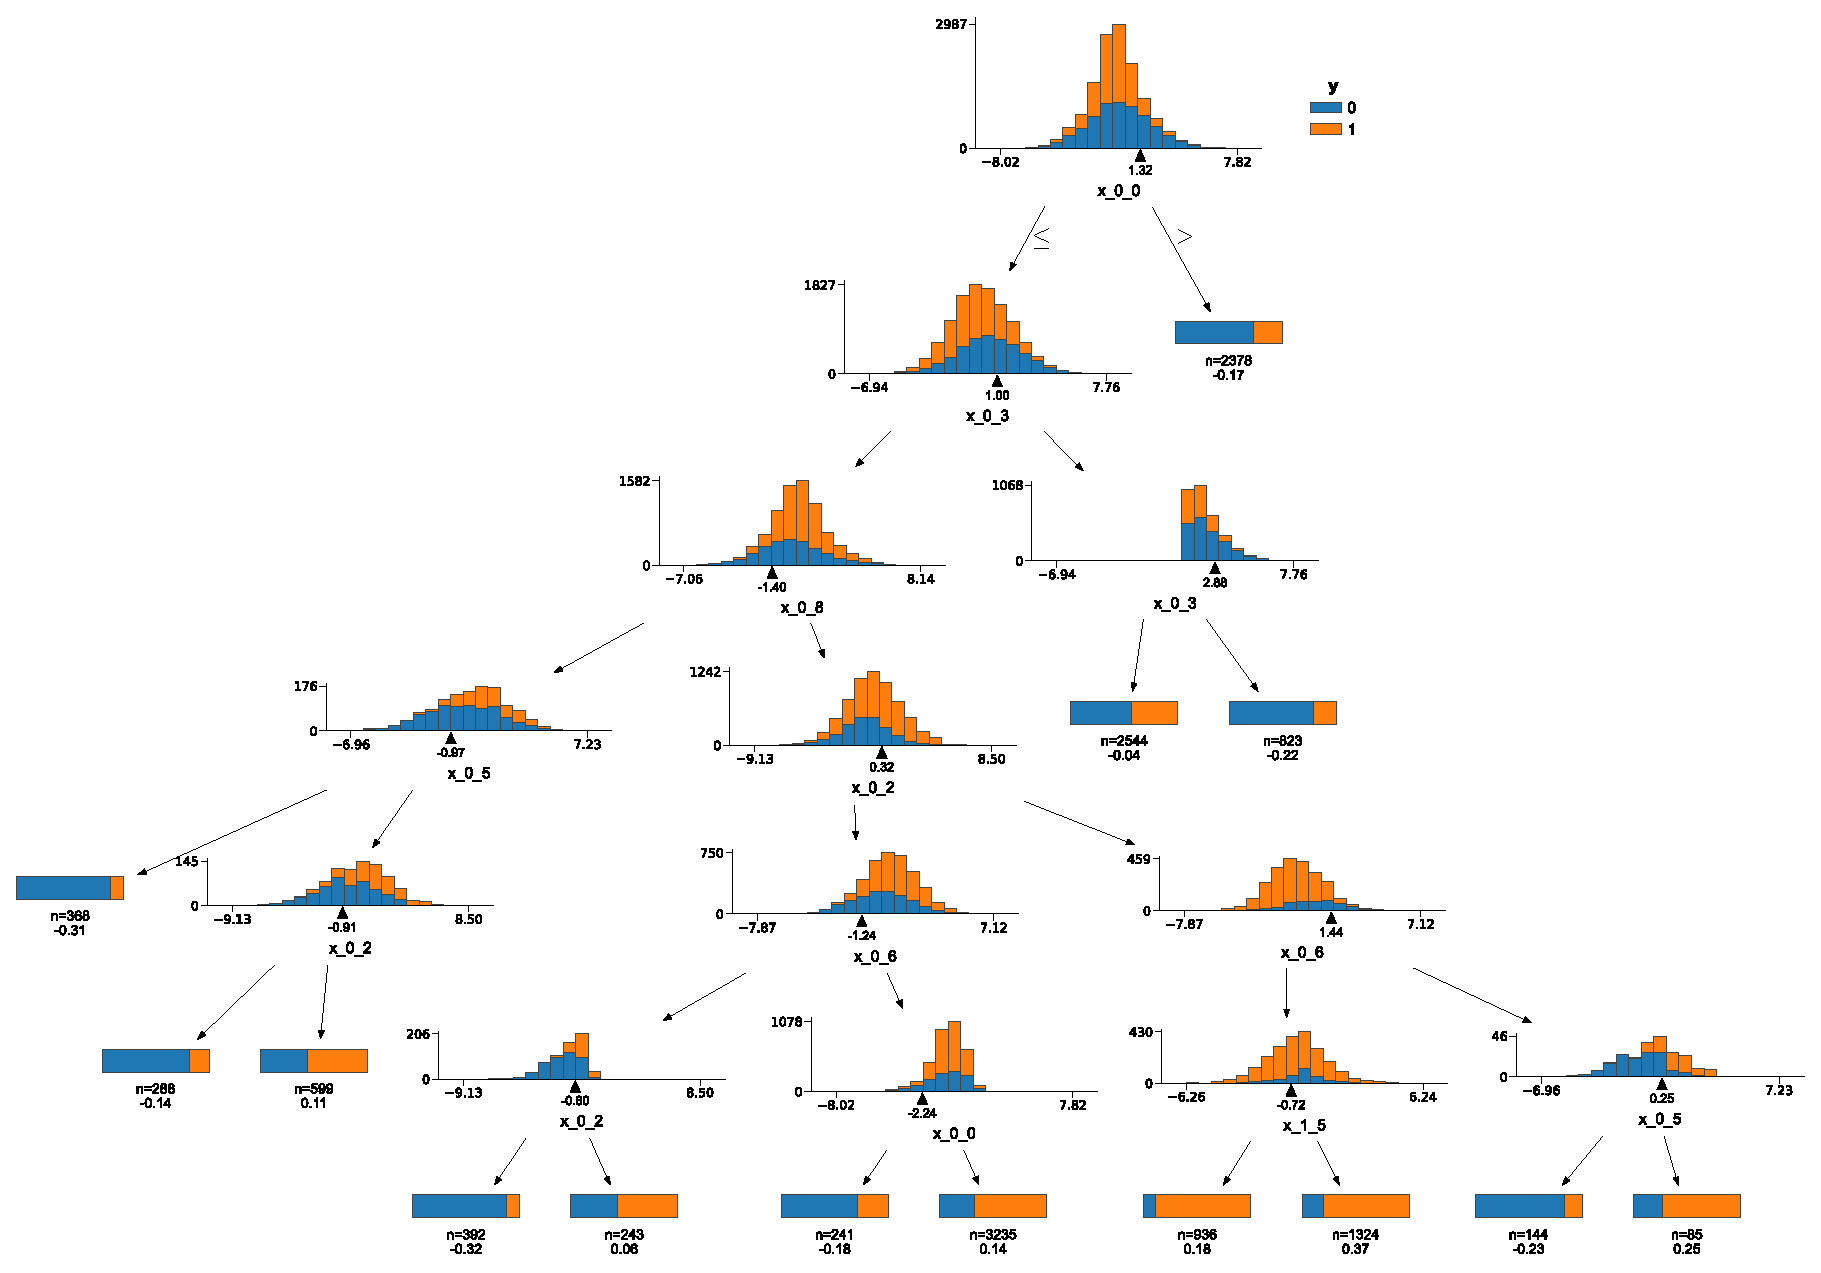
\includegraphics[width=\textwidth]{figures/ml/figs_demo/dtreeviz_figs_1}
  \caption{Tree 1}
  \label{fig:FIGS:demo_trees:tree1}
  \end{subfigure}
  ~
  \begin{subfigure}[b]{0.32\linewidth}\centering
      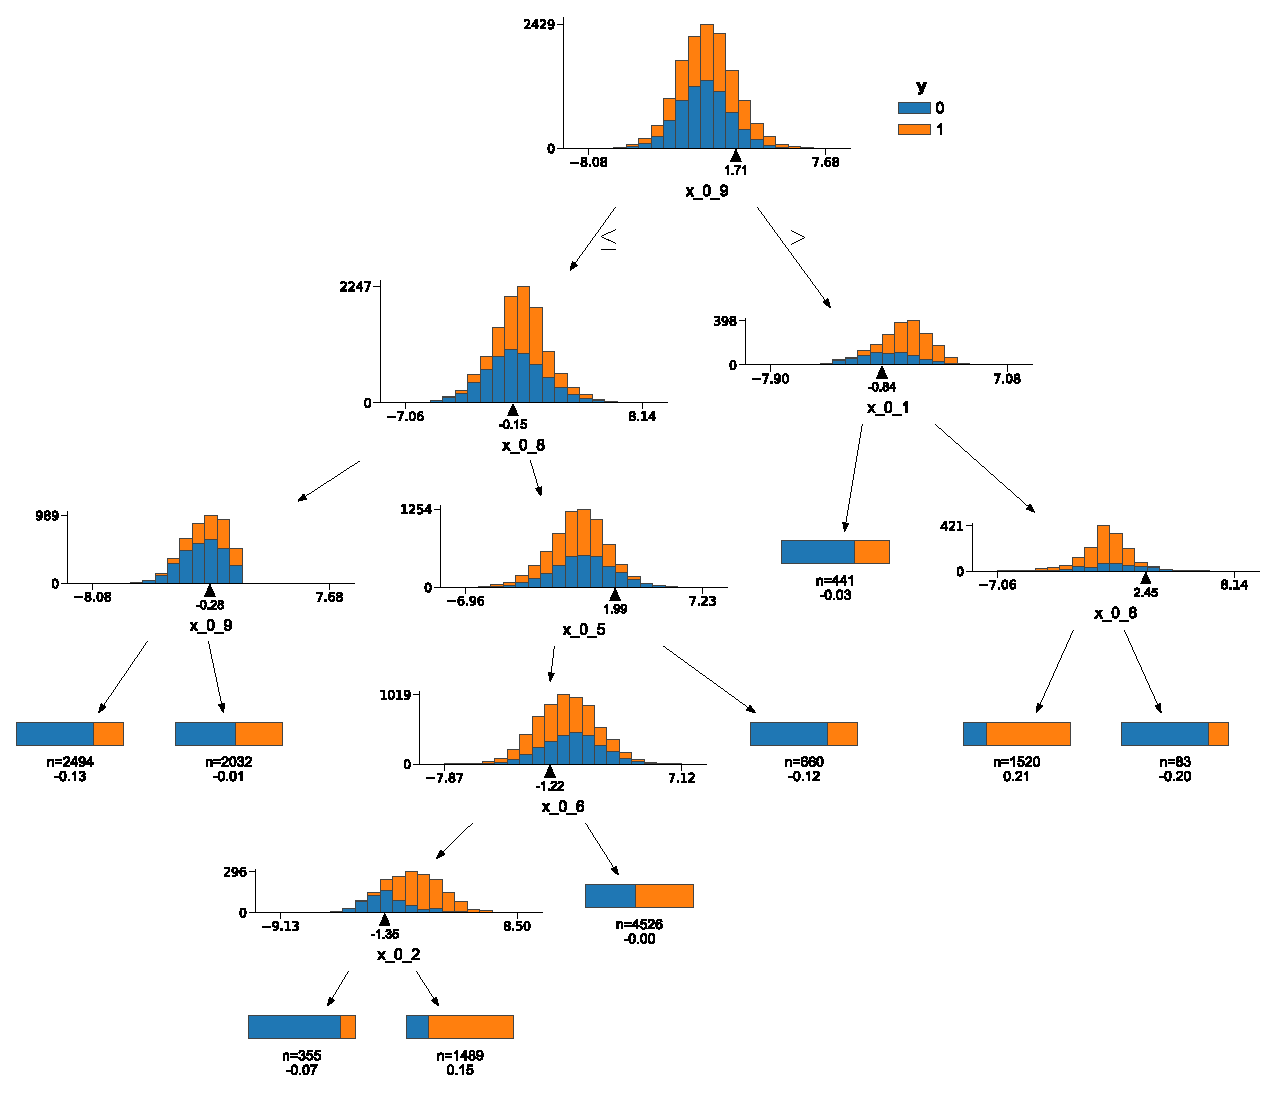
\includegraphics[width=\textwidth]{figures/ml/figs_demo/dtreeviz_figs_2}
  \caption{Tree 2}
  \label{fig:FIGS:demo_trees:tree2}
  \end{subfigure}
\caption{
The \figs model as trained on synthetic data in the
\texttt{figs\_demo.ipynb} \href{https://github.com/mepland/data_science_notes/blob/main/plots/figs_demo.ipynb}{notebook}.
Tree visualizations were created with the \texttt{dtreeviz} \href{https://github.com/parrt/dtreeviz}{package}.
The relatively small number of splits, \num{30}, and trees, \num{3}, make the \figs model readily interpretable.
In this case, the \figs model was able to learn the additive structure of the data,
as can be seen by each tree primarily splitting on a single MC generator $i$,
as shown in the feature names \texttt{x\_i\_j}.
To make predictions for $\vb{x}$, the weights at each terminating node are summed to create $P\left(y=1\right)$.
\label{fig:FIGS:demo_trees}
}
\end{figure}
\end{landscape}

\newpage

\begin{figure}[H]
  \centering
  \begin{subfigure}[b]{0.75\textwidth}\centering
      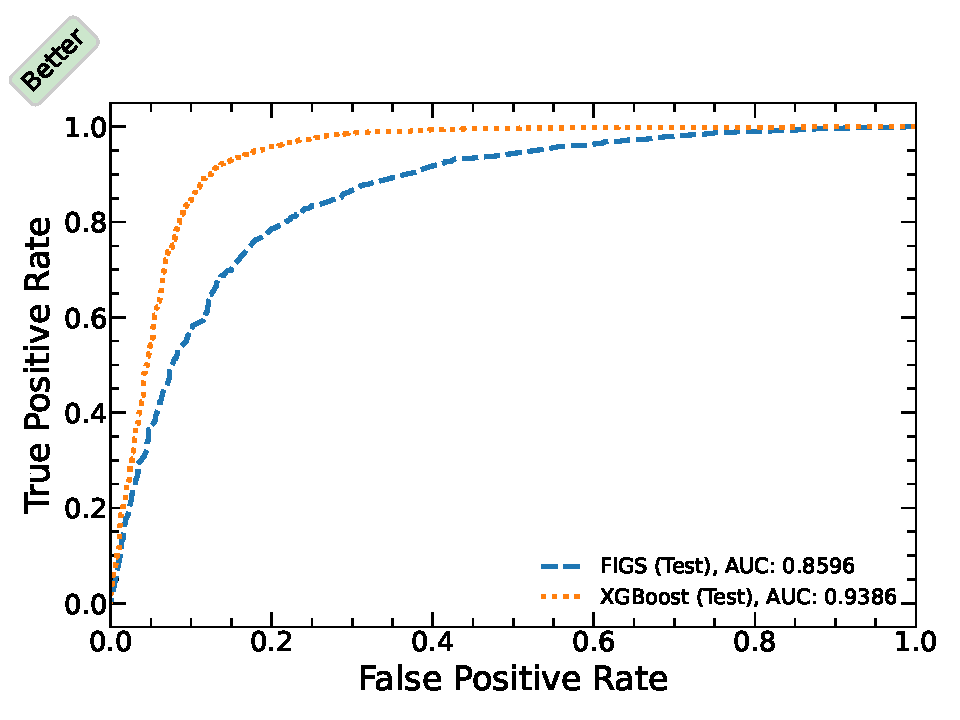
\includegraphics[width=\textwidth]{figures/ml/figs_demo/roc_figs_test_xgboost_test}
  \caption{\figs and \xgboost Test Set Comparison}
  \label{fig:FIGS:demo_roc:figs_xgboost}
  \end{subfigure}
  \newline
  \begin{subfigure}[b]{0.48\textwidth}\centering
      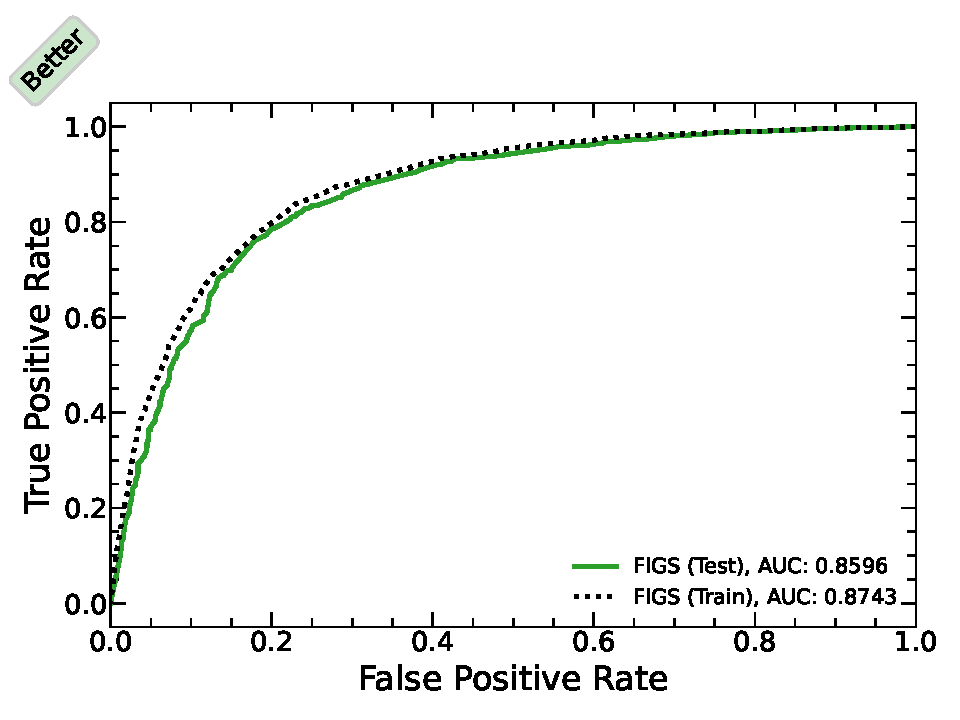
\includegraphics[width=\textwidth]{figures/ml/figs_demo/roc_figs_test_train}
  \caption{\figs}
  \label{fig:FIGS:demo_roc:figs}
  \end{subfigure}
  ~
  \begin{subfigure}[b]{0.48\textwidth}\centering
      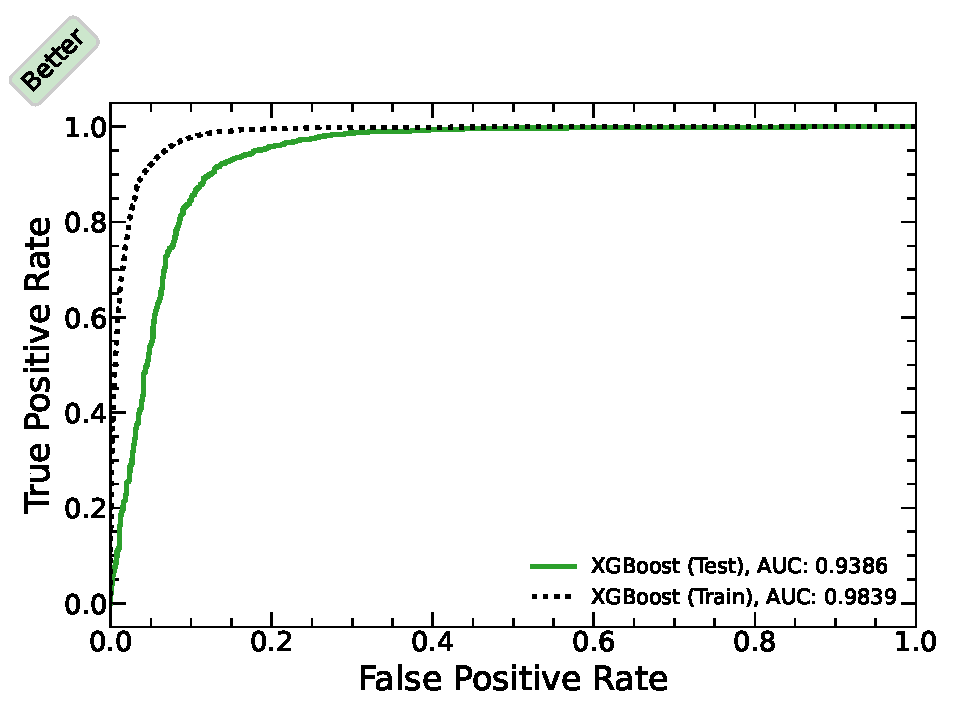
\includegraphics[width=\textwidth]{figures/ml/figs_demo/roc_xgboost_test_train}
  \caption{\xgboost}
  \label{fig:FIGS:demo_roc:xgboost}
  \end{subfigure}
\caption{
ROC curves for the \figs and \xgboost models trained in the
\texttt{figs\_demo.ipynb} \href{https://github.com/mepland/data_science_notes/blob/main/plots/figs_demo.ipynb}{notebook}.
While the \xgboost model has better performance, \mysubref{fig:FIGS:demo_roc:figs_xgboost},
the \figs model is much more interpretable and
is more consistent between train and test set performance, \mysubref{fig:FIGS:demo_roc:figs},
which should lead to less generalization error in production.
\label{fig:FIGS:demo_roc}
}
\end{figure}
